\begin{frame}{Motivations}

Soit $X$ un espace métrique dénombrable discret à géométrie bornée, i.e. $\sup_{x\in X} |B(x,R)|<\infty$ pour tout $R>0$. On note $H_X = l^2(X)\otimes H$ et 

\[C_R[X] = \{T\in \mathcal L(H_X) \text{ t.q. } T_{xy} \in \mathfrak K(H) \text{ et } prop(T) < R \}\]

\begin{definitionfr}[Algèbre de Roe]
\[C^*(X) = \overline{\cup_{R>0} C_R[X]} \subseteq \mathcal L(H_X).\]
\end{definitionfr}
\vspace{0.3 cm}
Si $X$ est une variété riemannienne non-compacte, $K(C^*(X))$ est le réceptacle pour les indices d'opérateurs différentiels elliptiques. (Approche développée par J. Roe)
\end{frame}

\begin{frame}{Motivations}
\begin{conj}[Baum-Connes coarse]
Soit $X$ un espace métrique dénombrable discret à géométrie bornée. Alors l'application d'assemblage
\[\mu_X : \varinjlim KK_*(C_0(P_d(X)),\C) \rightarrow K_*(C^*(X))\]
est un isomorphisme.
\end{conj}

Soit $\Gamma$ un groupe finiment engendré par une partie symmétrique $S$. \\
\vspace{0.3 cm}
On note $|\Gamma|$ l'espace métrique obtenu en munissant $\Gamma$ de la métrique de la longueur des mots. \\
\vspace{0.3 cm}
La conjecture de Baum-Connes coarse pour $|\Gamma |$ implique la conjecture de Novikov sur les hautes signatures associées à $\Gamma$. 
\end{frame}

\begin{frame}{Motivations}

\begin{thmfr}[Yu, 2010 \cite{Yu1}]
Soit $X$ de dimension asymptotique finie. Alors l'application d'assemblage
\[\mu_X : \varinjlim KK(C_0(P_d(X),\C) \rightarrow K(C^*(X))\]
est un isomorphisme.
\end{thmfr}
\vspace{0.3 cm}
Dans la preuve : des groupes d'obstruction notés $QP_{\delta, r ,s, k}(X)$ et $QU_{\delta, r ,s, k}(X)$ qui approximent la $K$-théorie. Ce sont les ancêtres de la $K$-théorie contrôlée.\\

\end{frame}

\begin{frame}{Motivations}

\begin{definitionfr}[Dimension asymptotique]
Un espace métrique est de dimension asymptotique $\leq d$ si, pour tout $R>0$, il existe un recouvrement $\mathcal U$ de $X$  tel que :
\vspace{0.3 cm}
\begin{itemize}
\item[$\bullet$] $\sup_{\mathcal U} diam(U)<\infty$ i.e. $\mathcal U$ est uniformément borné,
\vspace{0.3 cm}
\item[$\bullet$] $\mathcal U = \mathcal U_0 \coprod ... \coprod \mathcal U_d$ i.e. on peut colorier les ensembles par $d+1$ couleurs,
\vspace{0.3 cm}
\item[$\bullet$] $\inf_{U,U'\in\mathcal U_j} d(U,U')\geq R$, i.e. deux ensembles de la même couleur sont distants d'au moins $R$.
 \end{itemize}
\end{definitionfr}
\end{frame}

\begin{frame}{Motivations}
Par exemple, $asdim(\Z^2) \leq 2$.

\[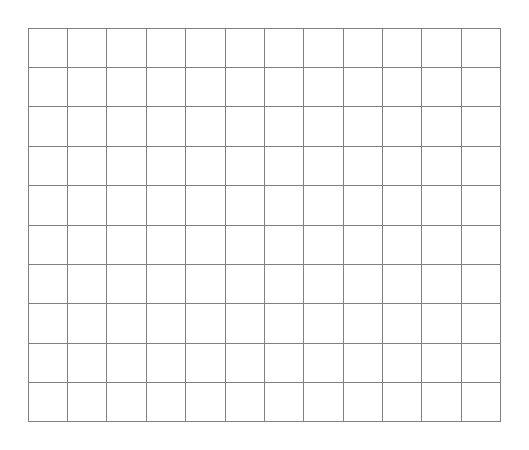
\begin{tikzpicture}
\draw [very thin, gray] (0,0) grid[step=0.5] (6,5);
\end{tikzpicture}\]
%\[\begin{tikzpicture}\foreach \x in {0,...,9}\draw  ( \x , 0) node {$\bullet$};\end{tikzpicture}\]
\end{frame}


\begin{frame}{Motivations}
Par exemple, $asdim(\Z^2) \leq 2$.
\[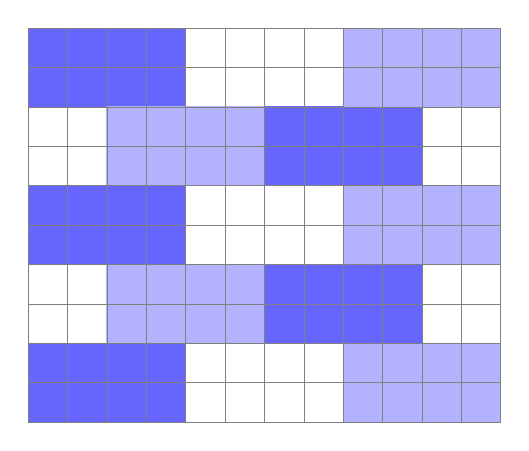
\begin{tikzpicture}

\draw[fill, blue!60] (0,0) rectangle (2,1) ; 
\draw[fill, blue!60] (0,2) rectangle (2,3) ; 
\draw[fill, blue!60] (0,4) rectangle (2,5) ; 
\draw[fill, blue!60] (3,1) rectangle (5,2) ;
\draw[fill, blue!60] (3,3) rectangle (5,4) ; 

\draw[fill, blue!30] (4,0) rectangle (6,1) ; 
\draw[fill, blue!30] (4,2) rectangle (6,3) ; 
\draw[fill, blue!30] (4,4) rectangle (6,5) ; 
\draw[fill, blue!30] (1,1) rectangle (3,2) ; 
\draw[fill, blue!30] (1,3) rectangle (3,4) ; 

\draw [very thin, gray] (0,0) grid[step=0.5] (6,5);
\end{tikzpicture}\]
%\[\begin{tikzpicture}\foreach \x in {0,...,9}\draw  ( \x , 0) node {$\bullet$};\end{tikzpicture}\]
\end{frame}

\begin{frame}{Motivations}
Par exemple, $asdim(\Z^2) \leq 2$.
\[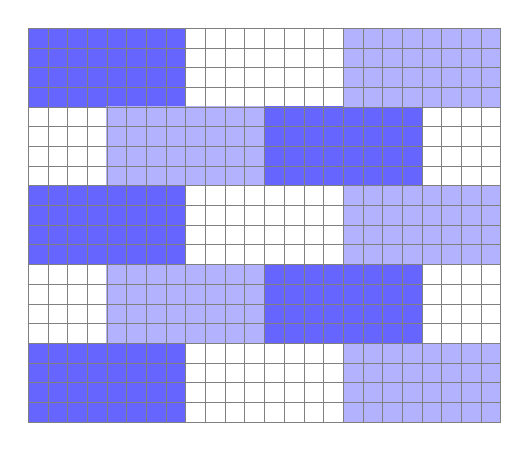
\begin{tikzpicture}

\draw[fill, blue!60] (0,0) rectangle (2,1) ; 
\draw[fill, blue!60] (0,2) rectangle (2,3) ; 
\draw[fill, blue!60] (0,4) rectangle (2,5) ; 
\draw[fill, blue!60] (3,1) rectangle (5,2) ;
\draw[fill, blue!60] (3,3) rectangle (5,4) ; 

\draw[fill, blue!30] (4,0) rectangle (6,1) ; 
\draw[fill, blue!30] (4,2) rectangle (6,3) ; 
\draw[fill, blue!30] (4,4) rectangle (6,5) ; 
\draw[fill, blue!30] (1,1) rectangle (3,2) ; 
\draw[fill, blue!30] (1,3) rectangle (3,4) ; 

\draw [very thin, gray] (0,0) grid[step=0.25] (6,5);
\end{tikzpicture}\]
%\[\begin{tikzpicture}\foreach \x in {0,...,9}\draw  ( \x , 0) node {$\bullet$};\end{tikzpicture}\]
\end{frame}

\begin{frame}{Motivations}
Par exemple, $asdim(\Z^2) \leq 2$.
\[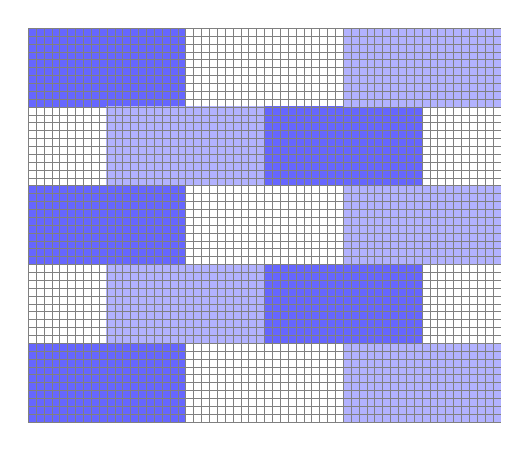
\begin{tikzpicture}

\draw[fill, blue!60] (0,0) rectangle (2,1) ; 
\draw[fill, blue!60] (0,2) rectangle (2,3) ; 
\draw[fill, blue!60] (0,4) rectangle (2,5) ; 
\draw[fill, blue!60] (3,1) rectangle (5,2) ;
\draw[fill, blue!60] (3,3) rectangle (5,4) ; 

\draw[fill, blue!30] (4,0) rectangle (6,1) ; 
\draw[fill, blue!30] (4,2) rectangle (6,3) ; 
\draw[fill, blue!30] (4,4) rectangle (6,5) ; 
\draw[fill, blue!30] (1,1) rectangle (3,2) ; 
\draw[fill, blue!30] (1,3) rectangle (3,4) ; 

\draw [very thin, gray] (0,0) grid[step=0.1] (6,5);
\end{tikzpicture}\]
%\[\begin{tikzpicture}\foreach \x in {0,...,9}\draw  ( \x , 0) node {$\bullet$};\end{tikzpicture}\]
\pause
Les groupes $QP_{\delta, r ,s, k}(X)$ et $QU_{\delta, r ,s, k}(X)$ satisfont une suite de Mayer-Vietoris qui n'existe pas en $K$-théorie.
\end{frame}

\begin{frame}{Motivations}

Un cadre plus général : la $K$-théorie quantitative (Oyono-Oyono \& Yu, 2015 \cite{OY2}) pour les $C^*$-algèbres filtrées.\\
\vspace{0.3 cm}
Une preuve plus générale :

\begin{thmfr}[Oyono-Oyono Yu, 2017]
Soit $X$ de décomposition géométrique finie. Alors l'application d'assemblage
\[\mu_X : \varinjlim KK(C_0(P_d(X),\C) \rightarrow K(C^*(X))\]
est un isomorphisme.
\end{thmfr}

\end{frame}
